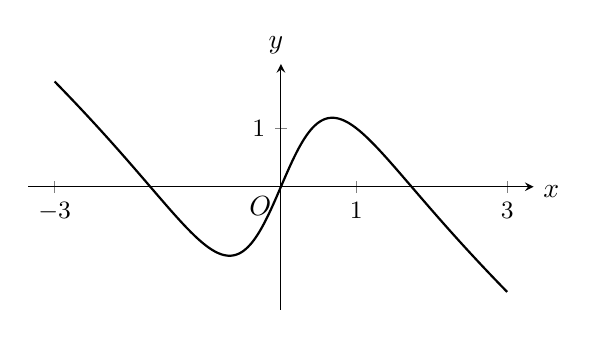
\begin{tikzpicture}
\begin{axis}[
  axis lines=middle,
  xmin=-3.35,xmax=3.35,
  ymin=-2.1,ymax=2.1,
  width=8cm,height=4.7cm,
  xtick={-3,0,1,3},
  xticklabels={$-3$,$O$,$1$,$3$},
  ytick={1},
  xlabel={$x$},ylabel={$y$},
  xlabel style={at={(axis description cs:1,.48)},anchor=west},
  ylabel style={at={(axis description cs:.49,1)},anchor=south},
  tick label style={font=\small},
  clip=true
]
\addplot[black,thick,samples=301,domain=-3:3] {(-x^3+3*x)/(x^2+1)};
\node[below left] at (axis cs:0,0) {$O$};
\end{axis}
\end{tikzpicture}
